\chapter{Proof-of-Concept}%
\label{ch:poc}
Voor het eerste praktische deel van deze bachelorproef werden er drie virtuele machines opgezet binnen VirtualBox met behulp van Vagrant om een gecontroleerde testomgeving te creëren. Deze virtuele machines (VM’s) simuleren een scenario waarin een ransomware-aanval gericht wordt op databases die door het bedrijf worden beheerd. Het primaire doel van deze simulatie is aan te tonen dat het gebruik van immutable storage een effectieve maatregel kan zijn om belangrijke data te beschermen tegen ransomware-aanvallen.
\subsection{Relevantie van de PoC voor de Azure-omgeving van Forvis Mazars}
De Proof-of-Concept (PoC) in VirtualBox simuleert een ransomware-aanval in een lokale omgeving, gericht op het evalueren van beveiligingsmaatregelen zoals immutable storage. Deze aanpak sluit nauw aan bij de Azure-omgeving van Forvis Mazars, waar databases en back-ups worden beheerd.

De technieken uit de PoC, zoals immutable storage, kunnen direct worden toegepast in Azure via functies zoals immutable blobs in Azure Storage. Dit maakt het mogelijk om gegevens beter te beschermen tegen wijzigingen of verwijdering. Daarnaast biedt de PoC een veilig platform om de impact van een ransomware-aanval te begrijpen en te testen hoe snel en effectief back-ups kunnen worden hersteld, wat een cruciaal aspect is voor de bedrijfscontinuïteit.

Forvis Mazars kan de PoC gebruiken om risico’s te analyseren en beveiligingsoplossingen eerst kleinschalig te testen, alvorens deze op grotere schaal binnen hun cloudinfrastructuur toe te passen. Hiermee helpt de PoC bij het verfijnen en optimaliseren van hun bestaande Azure-back-upstrategie.
\subsection{Technische uitwerking}
Voor het opzetten van de virtuele machines in de Proof-of-Concept (PoC) werd gebruik gemaakt van een Vagrantfile. De Vagrantfile definieert de specificaties en configuraties van de VM’s, zoals geheugen, CPU, netwerkadapters en besturingssysteem. 
\begin{lstlisting}[language=Ruby, caption={Vagrantfile voor drie VM's: Back-up Server, Client, en Attacker}]
Vagrant.configure("2") do |config|

# Primary VM
config.vm.define "primary" do |primary|
primary.vm.box = "ubuntu/jammy64"

primary.vm.network "private_network", ip: "192.168.0.10", virtualbox__intnet: "internal_network"

primary.vm.provider "virtualbox" do |vb|
vb.memory = "2048" 
vb.cpus = 1        
end
end

# Back-up VM
config.vm.define "backup" do |backup|
backup.vm.box = "ubuntu/jammy64"

backup.vm.network "private_network", ip: "192.168.0.20", virtualbox__intnet: "internal_network"

backup.vm.provider "virtualbox" do |vb|
vb.memory = "2048" 
vb.cpus = 1       
end
end

# Attacker VM
config.vm.define "attacker" do |attacker|
attacker.vm.box = "ubuntu/jammy64"

attacker.vm.network "private_network", ip: "192.168.0.30", virtualbox__intnet: "internal_network"

attacker.vm.provider "virtualbox" do |vb|
vb.memory = "1024" 
vb.cpus = 1        
end
end

end
\end{lstlisting}

In de onderstaande tabel worden de specificaties van de drie virtuele machines weergegeven die in de Proof-of-Concept zijn gebruikt. Elke VM heeft een specifieke functie binnen het netwerk. De tabel bevat details over de hoeveelheid toegewezen RAM, het aantal CPU-cores, het gebruikte besturingssysteem, de toegewezen IP-adressen en de configuratie van de netwerkadapter. Deze configuratie zorgt ervoor dat de VM's binnen hetzelfde interne netwerk met elkaar kunnen communiceren, wat essentieel is voor het testen van de ransomware-aanval en de back-upstrategieën.
\begin{longtable}{|l|c|c|c|l|l|}
    \hline
    \textbf{Functie} & \textbf{RAM} & \textbf{CPU Cores} & \textbf{IP} & \textbf{Besturingssysteem} & \textbf{Netwerkadapter} \\ \hline
    Primary server    & 2 GB         & 1                  & 192.168.0.10 & Ubuntu 22.04.5 LTS & NAT + Internal \\ \hline
    Back-up server           & 1 GB         & 1                  & 192.168.0.20 & Ubuntu 22.04.5 LTS & NAT + Internal \\ \hline
    Attacker VM         & 2 GB         & 1                  & 192.168.0.30 & Ubuntu 22.04.5 LTS     & NAT + Internal \\ \hline
    
\caption{Beschrijving van de virtuele machines in de Proof of Concept}
\end{longtable}

De Primary VM stelt een actieve databankserver voor binnen een bedrijfsomgeving. Deze server bevat de operationele data van het bedrijf en vertegenwoordigt de belangrijkste bron die beschermd moet worden tegen dataverlies of aanvallen. 

De Back-up VM fungeert als een back-upserver waarop regelmatig de databankback-ups worden opgeslagen. Deze back-upserver is cruciaal voor bedrijfscontinuïteit en disaster recovery, omdat ze in geval van een aanval of fout de herstelmogelijkheden biedt. 

De Attacker VM vertegenwoordigt een hacker met slechte intenties binnen de testomgeving. Deze machine wordt gebruikt om een ransomware-aanval te simuleren, waarbij de functionaliteit van zowel de Primary VM als de Back-up VM wordt bedreigd. Het doel van deze opstelling is om te demonstreren hoe een back-upstrategie, inclusief technieken zoals immutable storage, een bedrijf kan beschermen tegen de gevolgen van een dergelijke aanval.
\subsubsection{Aanmaken van de database}
Op de primary VM werd een eenvoudige SQL-database geïnstalleerd en de volgende tabel aangemaakt om als testdata te dienen:
\begin{lstlisting}[language=SQL, caption={MySQL-code voor het aanmaken van de testdatabank}]
CREATE TABLE employees (
    id INT AUTO_INCREMENT PRIMARY KEY,
    name VARCHAR(50),
    role VARCHAR(50)
);
INSERT INTO employees (name, role) VALUES 
    ('Alice', 'Engineer'), 
    ('Bob', 'Manager'), 
    ('Charlie', 'Analyst');
\end{lstlisting}



\subsubsection{Back-up van de database}
Nadien werd de database geëxporteerd naar een \texttt{.sql}-bestand met het volgende \texttt{mysqldump}-commando:
\begin{lstlisting}[language=bash, caption={mysqldump commando om een databank te exporteren}]
mysqldump -u testuser -p testdb > /home/vagrant/backup.sql
\end{lstlisting}
Het resulterende bestand, \texttt{backup.sql}, werd vervolgens met BorgBackup opgeslagen in een back-uprepository op de back-up VM. De repository werd vooraf geïnitialiseerd met het volgende commando:
\begin{lstlisting}[language=bash, caption={Borg commando om een map te initialiseren als Borg repository}]
borg init --encryption=repokey /home/vagrant/backups
\end{lstlisting}
Vervolgens werd de back-up gemaakt:
\begin{lstlisting}[language=bash, caption={Borg commando om een back-up te nemen}]
borg create --progress 
ssh://vagrant@192.168.0.20/home/vagrant/backups::backup-$(date +%Y-%m-%d) 
/home/vagrant/backup.sql
\end{lstlisting}

\subsubsection{Beveiliging van de back-updirectory}
Om de back-updirectory ransomware-resistent te maken, werd het Linux-commando \texttt{chattr} gebruikt om het \textit{immutable}-attribuut toe te passen op de back-updirectory. Dit attribuut zorgt ervoor dat er geen wijzigingen aan de bestanden in de directory gebeuren, zelfs door gebruikers met \texttt{root}-rechten. Het commando:
\begin{lstlisting}[language=bash, caption={Linux commando om de map immutable te maken}]
sudo chattr +i /home/vagrant/backups/
\end{lstlisting}

\subsubsection{Simulatie van de ransomware-aanval}
Op de attacker VM werd een script gebruikt om de ransomware-aanval te simuleren. Het script probeert alle bestanden in de back-updirectory te hernoemen door \texttt{.malware} toe te voegen aan de bestandsnamen. Dit zou overeenkomen met een ransomware-aanval waarbij de back-up bestanden geëncrypteerd worden. Het script is hieronder weergegeven:
\begin{lstlisting}[language=bash, caption={Bash script om een ransomware-aanval na te bootsen}]
#!/bin/bash
    
BACKUP_DIR="/home/vagrant/backups"
    
for file in "$BACKUP_DIR"/*; do
  if [ -f "$file" ]; then
    if mv "$file" "${file}.malware"; then
      echo "Renamed $file to ${file}.malware"
    else      
      echo "Error: Could not rename $file"    
    fi    
  fi    
done    
\end{lstlisting}
Voor het gemak heeft de Attacker VM volledige controle gekregen over de Back-up VM. Dit is gedaan omdat de scope van deze bachelorproef niet is om toegang te verkrijgen tot een server, maar eerder om een gecontroleerde omgeving te creëren waarin een Attacker VM een ransomware-aanval nabootst. Het doel is te demonstreren hoe de ransomware zich verspreidt naar de back-up directory, en niet om de daadwerkelijke methoden voor het verkrijgen van toegang tot een server in detail uit te werken.

Toen dit script werd uitgevoerd op de back-up VM, werd duidelijk dat het hernoemen van de bestanden niet lukte vanwege het immutable-attribuut. Dit toont aan dat de ransomware-aanval niet slaagde en de bestanden in de back-updirectory beschermd bleven.

\subsubsection{Herstellen van de back-ups}
Om te bewijzen dat de back-ups nog steeds bruikbaar waren, werd een herstelproces uitgevoerd op de primary VM vanuit de Borg-repository:
\begin{lstlisting}[language=bash, caption={Borg commando om een back-up te herstellen}]
borg extract 
ssh://vagrant@192.168.0.20/home/vagrant/backups::backup-2024-12-05
\end{lstlisting}

De databank werd opnieuw opgezet vanuit het bestand dat uit de Borg-repository werd gehaald met het volgende commando:
\begin{lstlisting}[language=bash, caption={MySQL commando om een databank te herstellen vanuit een .sql-bestand}]
mysql -u root -p restored_db < /home/vagrant/backup.sql
\end{lstlisting}
De back-up werd gebruikt om de database te herstellen en te controleren. Het herstelproces verliep succesvol, wat bewijst dat de immutable storage de integriteit van de back-ups had behouden en dat de bestanden veilig waren gebleven ondanks de ransomware-aanval.

\newpage
\subsection{Implementatie van immutable storage in de Azure-omgeving}
\subsubsection{Aanmaken van een storage account}
De eerste stap in het implementeren van Immutable Storage in Azure is het aanmaken van een \texttt{Storage Account} in de Azure Portal. 
\begin{figure}[h]
    \centering
    \captionsetup{justification=centering}    
    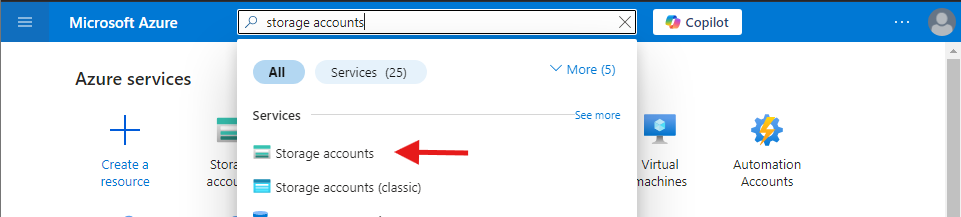
\includegraphics[width=0.8\textwidth]{img/1imm.png}
    \caption{Storage account zoekopdracht binnen de Azure Portal}
\end{figure}
Bij het aanmaken van het storage account kiezen we de correcte resource group, naam die het account moet krijgen, regio en bij redundancy kiezen we voor \texttt{Locally-redundant storage (LRS)}. Bij de optie \texttt{Account kind} kiezen we voor \texttt{General-purpose v2}, omdat deze versie alle benodigde functionaliteit biedt, zoals het ondersteunen van de blob storage en het configureren van immutability policies. 
\begin{figure}[h]
    \centering
    \captionsetup{justification=centering}    
    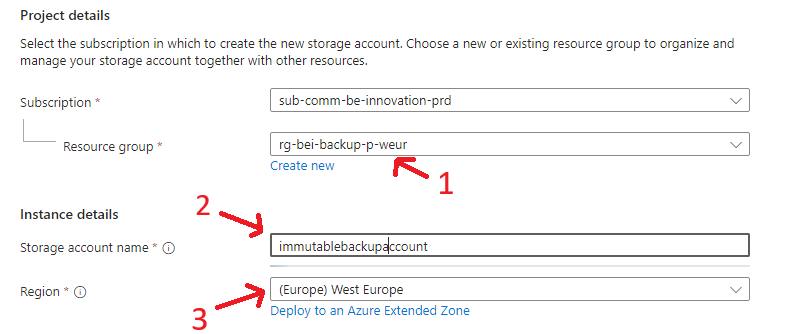
\includegraphics[width=0.8\textwidth]{img/3.1imm.png}
    \caption{Configuratie voor het nieuwe storage account}
\end{figure}
\begin{figure}[h]
    \centering
    \captionsetup{justification=centering}    
    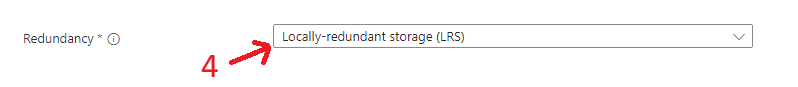
\includegraphics[width=0.8\textwidth]{img/3.2imm.png}
    \caption{Tweede deel van de configuratie voor het nieuwe storage account}
\end{figure}
\newpage
\subsubsection{Aanmaken van een container binnen het storage account}
Na het aanmaken van het storage account moet er een container geconfigureerd worden binnen het nieuwe storage account om de gegevens op te slaan. Bij het aanmaken van de container moet de \texttt{public access level} op private staan voor de veiligheid. Containers in Azure werken als mappen waarin je blobs kunt opslaan zoals back-ups.
\begin{figure}[h]
    \centering
    \captionsetup{justification=centering}    
    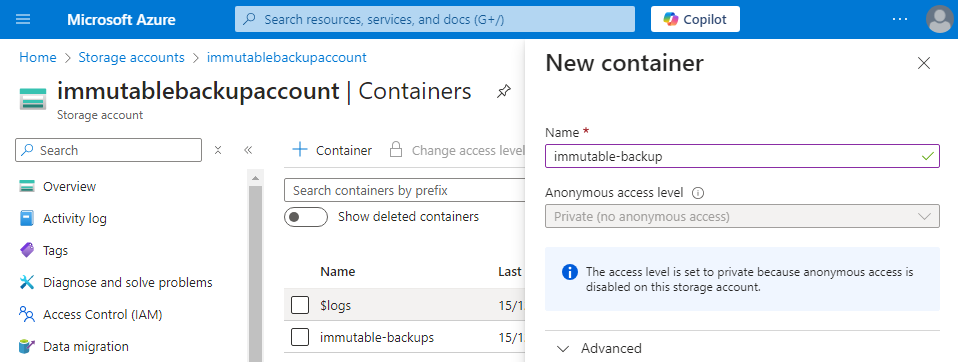
\includegraphics[width=0.8\textwidth]{img/4imm.png}
    \caption{Configuratie voor de container in het storage account}
\end{figure}
\subsubsection{Opzetten van een time-based retention policy}
Nadien moet er een immutability policy opgezet worden. Hierbij werd gekozen voor een time-based retention policy van 90 dagen, de back-up is met andere woorden bescherm tegen verwijdering of wijziging voor deze periode. Dit is een veilige en praktische keuze voor back-ups. Daarnaast is er bij de optie \texttt{ Allow protected append writes to } gekozen voor \texttt{ Block and append blobs}, dit maakt het mogelijk om gegevens te blijven toevoegen aan de blob zonder de bestaande gegevens te wijzigen of te verwijderen, wat ideaal is voor scenario's zoals logbestanden of incrementele back-ups.
\begin{figure}[h]
    \centering
    \captionsetup{justification=centering}    
    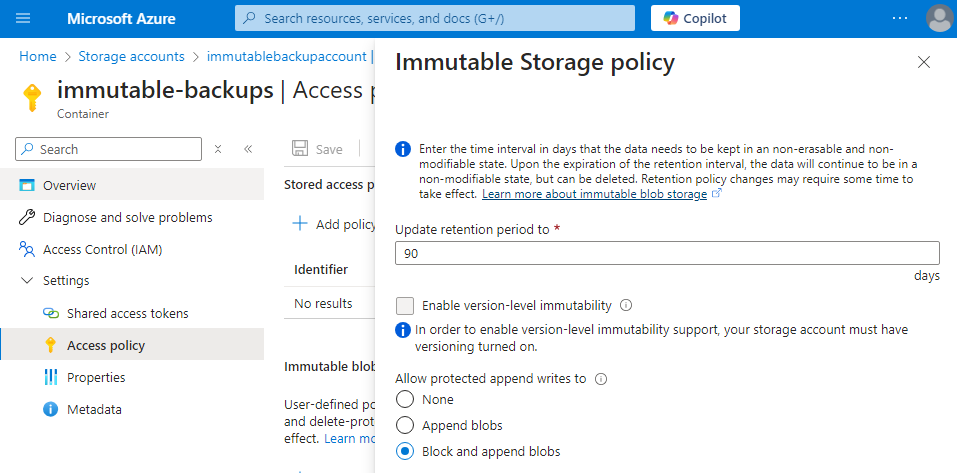
\includegraphics[width=0.8\textwidth]{img/6imm.png}
    \caption{Configuratie voor time-based retention policy}
\end{figure}
\newpage
\subsubsection{Testen van de immmutable storage}
Om de immutable storage te testen is er gekozen om een back-up van een MySQL-database de uploaden naar de container. Na het uploaden van het bestand was er geen optie om dit bestand te verwijderen of te wijzigen. Met andere woorden is deze back-up dus beschermd tegen een ransomware-aanval.
\begin{figure}[h]
    \centering
    \captionsetup{justification=centering}    
    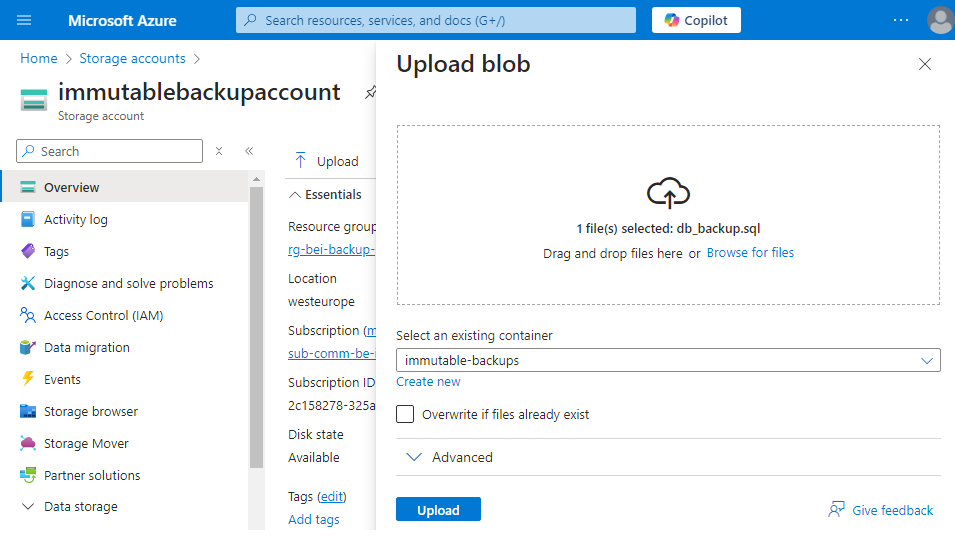
\includegraphics[width=0.8\textwidth]{img/7imm.png}
    \caption{Uploaden van het back-up bestand van de MySQL-databank}
\end{figure}
\begin{figure}[h]
    \centering
    \captionsetup{justification=centering}    
    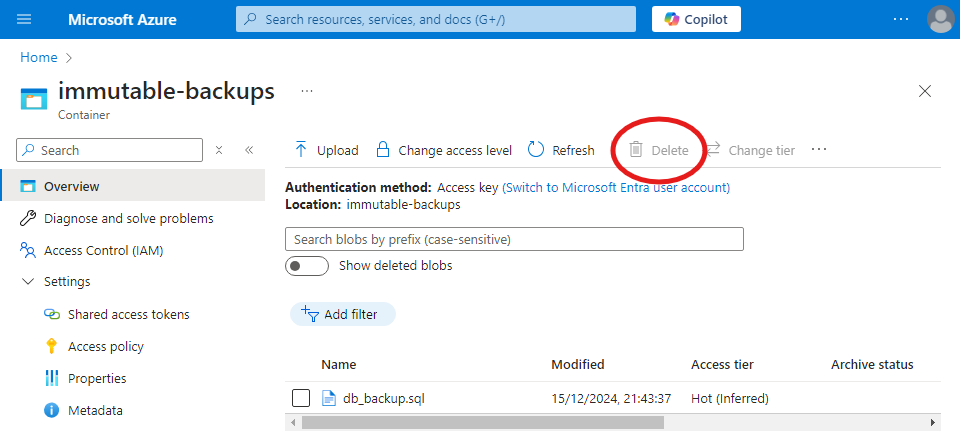
\includegraphics[width=0.8\textwidth]{img/8imm.png}
    \caption{Screenshot van de poging om het bestand te verwijderen, waarbij de actie wordt geblokkeerd}
\end{figure}
\subsubsection{Conclusie}
De implementatie van immutable storage op het azure storage account is succesvol afgerond, waardoor de opgeslagen back-ups nu beschermd zijn tegen onverwachte wijzigingen of verwijderingen. Daarnaast worden er dagelijks automatische back-ups van de databanken genomen, welke een retentieperiode van 7 dagen hebben. Dit zorgt ervoor dat er altijd een versie van de back-up beschikbaar is, zelfs als de meest recente back-up beschadigd of onbruikbaar blijkt. Deze combinatie van immutable storage en versiebeheer versterkt de bescherming tegen dataverlies en maakt het mogelijk om eerdere, werkende back-ups snel te herstellen.





































